% =====================================================================
%  Fig. 3 -- Residual Dual-Pooling Graph Reasoning Branch
% =====================================================================
\documentclass[tikz,border=3pt]{standalone}
\usepackage{helvet}
\renewcommand{\familydefault}{\sfdefault}
\usepackage{amsmath,amssymb}
\usetikzlibrary{arrows.meta,positioning,calc,fit,backgrounds,decorations.pathreplacing}

\hyphenpenalty=10000 \exhyphenpenalty=10000 \pretolerance=10000 \tolerance=9999

\definecolor{cGraph}{HTML}{5B4B8A}  \definecolor{cGraphBg}{HTML}{ECE8F6}
\definecolor{cFuse}{HTML}{9E2A2B}   \definecolor{cFuseBg}{HTML}{F8E5E5}
\definecolor{cPool}{HTML}{2A6F97}   \definecolor{cPoolBg}{HTML}{E3EEF5}
\definecolor{cInk}{HTML}{1F2933}

\begin{document}
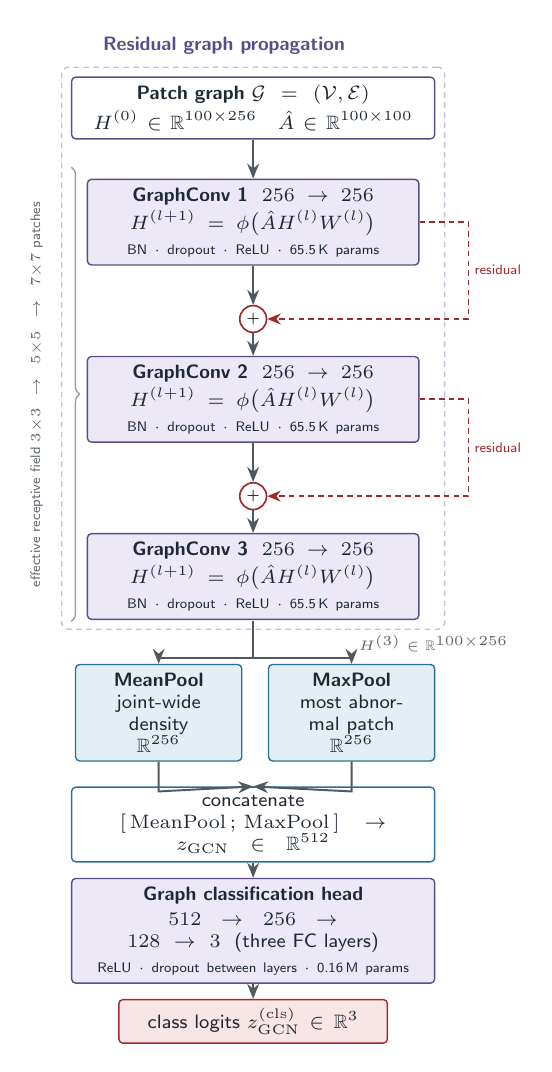
\begin{tikzpicture}[
  font=\scriptsize,
  blk/.style 2 args={draw=#1, fill=#2, rounded corners=1.5pt, line width=.5pt,
                     align=center, text=cInk, inner sep=3pt},
  flow/.style={-{Stealth[length=1.9mm,width=1.5mm]}, line width=.7pt, draw=cInk!78},
  res/.style={-{Stealth[length=1.7mm,width=1.4mm]}, line width=.65pt, draw=cFuse,
              dash pattern=on 2pt off 1.5pt},
  shp/.style={font=\tiny, text=cInk!72, inner sep=1pt},
  ttl/.style={font=\scriptsize\bfseries, text=cGraph},
  panel/.style={draw=cGraph!35, rounded corners=2.5pt, line width=.5pt,
                dash pattern=on 2pt off 1.6pt},
  add/.style={circle, draw=cFuse, fill=white, line width=.6pt,
              inner sep=0pt, minimum size=3.4mm, font=\tiny},
]

% ---------------- input ----------------
\node[blk={cGraph}{white}, text width=44mm] (in) at (2.65,10.30)
  {\textbf{Patch graph} $\mathcal{G}=(\mathcal{V},\mathcal{E})$\\[1pt]
   $H^{(0)}\in\mathbb{R}^{100\times256}$\quad $\hat{A}\in\mathbb{R}^{100\times100}$};

% ---------------- three graph-conv layers ----------------
\newcommand{\gcnlayer}[3]{%
  \node[blk={cGraph}{cGraphBg}, text width=40mm] (#1) at (2.65,#2)
    {\textbf{GraphConv #3}\ \ $256 \rightarrow 256$\\[1pt]
     $H^{(l+1)}=\phi\big(\hat{A}H^{(l)}W^{(l)}\big)$\\[1pt]
     {\tiny BN $\cdot$ dropout $\cdot$ ReLU $\cdot$ 65.5\,K params}};}

\gcnlayer{g1}{8.85}{1}
\node[add] (s2) at (2.65,7.62) {$+$};
\gcnlayer{g2}{6.60}{2}
\node[add] (s3) at (2.65,5.37) {$+$};
\gcnlayer{g3}{4.35}{3}

\draw[flow] (in) -- (g1);
\draw[flow] (g1) -- (s2);
\draw[flow] (s2) -- (g2);
\draw[flow] (g2) -- (s3);
\draw[flow] (s3) -- (g3);

% residual skips around layers 2 and 3
\draw[res] (g1.east) -- ++(0.62,0) |- (s2.east);
\draw[res] (g2.east) -- ++(0.62,0) |- (s3.east);
\node[shp, text=cFuse, anchor=west] at (5.42,8.24) {residual};
\node[shp, text=cFuse, anchor=west] at (5.42,5.99) {residual};

% receptive-field annotation
\draw[decorate, decoration={brace, amplitude=3pt}, draw=cInk!45, line width=.5pt]
  (0.34,9.55) -- (0.34,3.78);
\node[shp, rotate=90, anchor=south, text width=58mm, align=center] at (0.02,6.66)
  {effective receptive field
   $3{\times}3 \rightarrow 5{\times}5 \rightarrow 7{\times}7$ patches};

% ---------------- dual pooling ----------------
\node[shp, anchor=west] at (3.95,3.50) {$H^{(3)}\in\mathbb{R}^{100\times256}$};

\node[blk={cPool}{cPoolBg}, text width=19mm] (mean) at (1.45,2.62)
  {\textbf{MeanPool}\\ joint-wide density\\ $\mathbb{R}^{256}$};
\node[blk={cPool}{cPoolBg}, text width=19mm] (max) at (3.90,2.62)
  {\textbf{MaxPool}\\ most abnormal patch\\ $\mathbb{R}^{256}$};

\draw[flow] (2.65,3.78) -- (2.65,3.32) -- (1.45,3.32) -- (mean.north);
\draw[flow] (2.65,3.78) -- (2.65,3.32) -- (3.90,3.32) -- (max.north);

\node[blk={cPool}{white}, text width=44mm] (cat) at (2.65,1.20)
  {concatenate $\;[\,\mathrm{MeanPool}\,;\,\mathrm{MaxPool}\,]\;
   \rightarrow\; z_{\mathrm{GCN}}\in\mathbb{R}^{512}$};
\draw[flow] (mean.south) -- (1.45,1.62) -- (cat.north);
\draw[flow] (max.south) -- (3.90,1.62) -- (cat.north);

% ---------------- classification head ----------------
\node[blk={cGraph}{cGraphBg}, text width=44mm] (head) at (2.65,-0.15)
  {\textbf{Graph classification head}\\[1pt]
   $512 \rightarrow 256 \rightarrow 128 \rightarrow 3$\ \ (three FC layers)\\[1pt]
   {\tiny ReLU $\cdot$ dropout between layers $\cdot$ 0.16\,M params}};
\draw[flow] (cat) -- (head);

\node[blk={cFuse}{cFuseBg}, text width=32mm] (out) at (2.65,-1.30)
  {class logits $z^{(\mathrm{cls})}_{\mathrm{GCN}}\in\mathbb{R}^{3}$};
\draw[flow] (head) -- (out);

\begin{scope}[on background layer]
  \node[panel, fit=(in)(g1)(g2)(g3)(s2)(s3)] {};
\end{scope}
\node[ttl, anchor=south west] at (0.62,10.86) {Residual graph propagation};

\end{tikzpicture}
\end{document}
